%
%  This document contains chapter 3 of the thesis.
%

\chapter{RESULTS}\label{ch:results}
This chapter attempts to answer the questions previously outlined in the
\hyperref[subsec:analysis]{Analysis} section.
Each section is dedicated to exploring one question.
The process used is described in each section though the process usually
consists of using a combination of graphing, One-way ANOVA tests, and
Student's t- or Mann-Whitney U-tests.
All tests are performed with $\alpha = 0.05$ unless otherwise stated.

\section{Lowest Error Voting Mechanisms}\label{sec:lowest-error-voting-mechanism}
Voting mechanisms consolidate the votes of all agents along with their weights
into a final estimate, and so play a pivotal role in the accuracy of a system.
\autoref{fig:voting-mechanisms-comparison} illustrates the population of
squared error for each voting mechanism.

\begin{figure}[htbp]
    \centering
    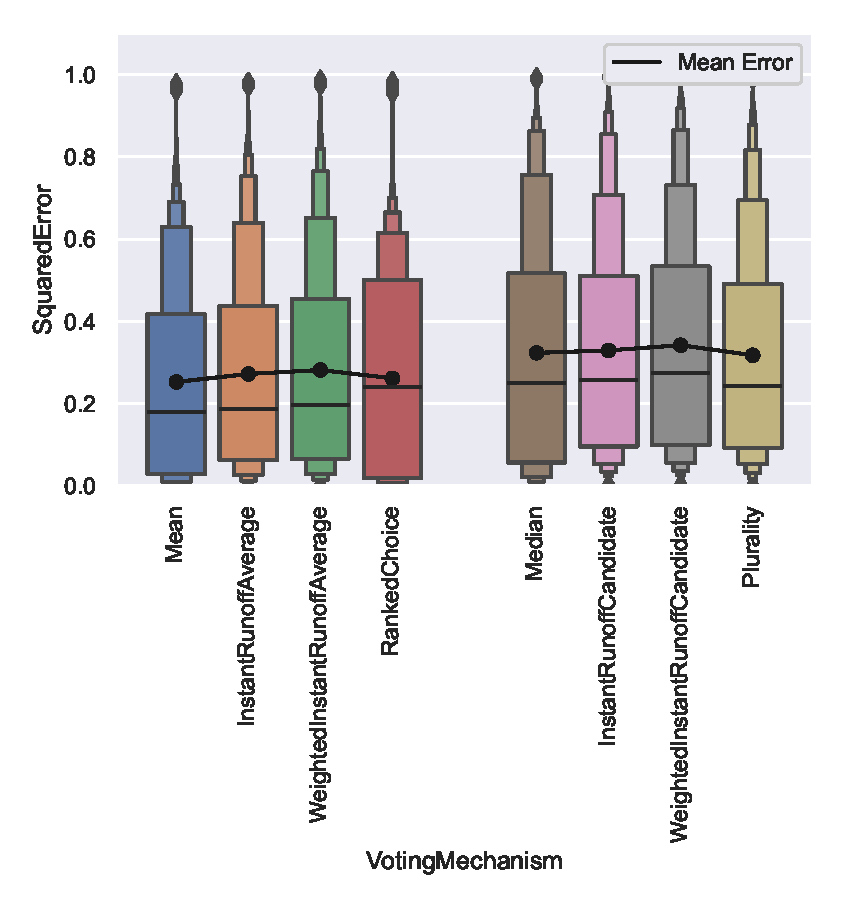
\includegraphics[scale=0.75]
    {./content/figures/voting_mechanisms_comparison}
    \caption{Squared error populations by voting mechanism, with average
    mechanisms on the left and candidate mechanisms on the right.}
    \label{fig:voting-mechanisms-comparison}
\end{figure}

This graph immediately tells us a few things.
First, the squared error seems to be skewed, favoring numbers closer to 0.
This means there is a fairly even spread of estimates, since this is the
pattern one would expect to see from a uniform distribution of estimates.
Interestingly, however, is the majority of most error populations are
somewhere between a uniform distribution of estimates
(\autoref{fig:expected_even_distribution_squared_error}) and a normal
distribution (\autoref{fig:expected_gaussian_distribution_squared_error}).
Indeed, if the estimates are instead graphed as in
\autoref{fig:voting_mechanisms_estimate_distribution}, the distribution of estimates
is more normal than uniform.
This means most mechanisms are better at estimating \truth\ than random chance.

Additionally, while all distributions appear generally close, there appears to be a
slight difference between average and candidate mechanisms.
This can be confirmed by comparing the average mechanisms to the candidate mechanisms
using a Mann-Whitney U-test, with the alternative being the average mechanisms'
squared error is lesser.
Performing such a test results in a p-value of 0.0, far below the $\alpha$ of 0.05.
Since candidate mechanisms can still be useful depending on the situation, both the
best average mechanisms and the best candidate mechanisms will be identified.

Further U-tests were performed, comparing each individual voting mechanism against
every other individual mechanism.
The results of this analysis can be found in
\autoref{fig:all-voting-mechanisms-p-values}, and is further segmented and discussed in
\autoref{subsec:lowest-error-average-mechanisms} and
\autoref{subsec:lowest-error-candidate-mechanisms}.

\subsection{Average Mechanisms}\label{subsec:lowest-error-average-mechanisms}

\subsection{Candidate Mechanisms}\label{subsec:lowest-error-candidate-mechanisms}


\section{Best Overall Weighting Mechanism}\label{sec:best-overall-weighting-mechanism}


\section{Best Overall Combination}\label{sec:best-overall-combination}


\section{Best Inactive to Proxy Ratio}\label{sec:best-inactive-to-proxy-count}


\section{Caveat}\label{sec:caveat}
% Explain how WeightlessAverageAll works best
% TODO: Try to find some cirumstance where some else works better

